
%%%%%%%%%%%%%%%%%%%%%%%%%%%%%%%%%%%%%%%%%%%%%%%%
%%%%%%%%%%%%%%%%%%%%%%%%%%%%%%%%%%%%%%%%%%%%%%%%       
    \section{Identity, Privacy  and Sovereignty }
    \frame{\sectionpage}
    \subsection{Identity}
%%%%%%%%%%%%%%%%%%%%%%%%%%%%%%%%%%%%%%%%%%%%%%%%    
    \begin{frame}{Identity}
     
%      \begin{definition}[Wikipedia]
%      Identity is the qualities, beliefs, personality traits, appearance, and/or expressions that characterize a person or group.
%      \end{definition}
     
        \only<1>{ 
          \begin{definition}[Wikipedia]
     Identity is the qualities, beliefs, personality traits, appearance, and/or expressions that characterize a person or group.
     \end{definition}
        }
        \only<2>{
        \begin{definition}[{[CL16]}]
      Digital identity is a collection of attributes someone knows about.
     \end{definition}
     \begin{center}
     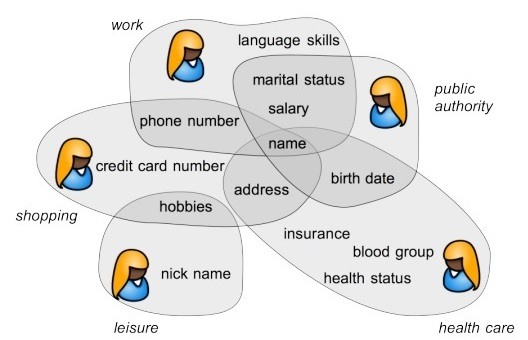
\includegraphics[width=7.5cm]{images/identity.jpg}
     \end{center}
     From now on we will refer Identity, Privacy and Sovereignty as Digital ones.
        }
    
    \end{frame}

%%%%%%%%%%%%%%%%%%%%%%%%%%%%%%%%%%%%%%%%%%%%%%%%

    \subsection{Privacy}
    \begin{frame}{Privacy}
    
    \begin{definition}[Wikipedia]
    Privacy is the ability of an individual or group to seclude {\color{blue2}{themselves}} or {\color{red}{information}} about themselves, and thereby express themselves {\color{red}selectively}.
    \end{definition}
 
    \begin{block}{Vires in Numeris}
    \only<1>
    {
     \begin{tabular}{ll}
        \begin{minipage}{4cm}
         ~\\~\\~\\~\\
        \end{minipage}
        &
        \begin{minipage}{5.5cm}
         ~\\~\\~\\~\\
        \end{minipage}
      \end{tabular}  
    }
    \only<2-3>
    {
    \begin{tabular}{ll}
        \begin{minipage}{4cm}
          
\includegraphics[width=4cm]{images/privacy.jpeg}
        \end{minipage}
        &
        \begin{minipage}{5.5cm}
         \begin{itemize}
          \item Alphabet+Meta : 3G€
          \item Nym's Fund : 0.3 G€
          \item RGPD : 1G€ in France
         \end{itemize}

        \end{minipage}
    \end{tabular}  
    }
    \end{block}
    
    
     \only<1-2>
    {
    \begin{exampleblock}{Definition (IND-PRIV2)}
     \begin{tabular}{ll}
        \begin{minipage}{4cm}
         ~\\~\\~\\~\\
        \end{minipage}
        &
        \begin{minipage}{5.5cm}
        ~\\~\\~\\~\\
        \end{minipage}
      \end{tabular}  
      \end{exampleblock}
    }
    \only<3>
    {
    \begin{alertblock}{Definition (IND-PRIV2)}
     
   
    \begin{tabular}{ll}
        \begin{minipage}{4cm}
          \includegraphics<3>[width=4cm]{images/blackhole.jpg}
        \end{minipage}
        &
        \begin{minipage}{5.5cm}
         \begin{itemize}
          \item Privacy domain is unclear : no RGS or unique primitive
          \item Survey (Kahoot)
         \end{itemize}
        \end{minipage}
    \end{tabular}  
    
    \end{alertblock}

     }
    
    \end{frame}
    %Selon une étude de la CDC, 21 % des internautes fournissent volontairement des données erronées
      %404 : Not Found
%%%%%%%%%%%%   
  \begin{frame}{Privacy at Ledger}
  
  \begin{block}{Use cases}
    \begin{itemize}
     \item Ledger Database : update of Ledger Live links accounts
     \item Device ID : links desktops and phones
     \item Ledger Live :  genuine check
     \item Registering to a conference with Ether Fee
    \end{itemize}
    \end{block}
   
   \begin{alertblock}{Noob Remarks}
    \begin{itemize}
     \item We have privacy legal, but no privacy tech's or dungeon
     
    \end{itemize}   
   \end{alertblock}

   Take offline solutions as priority, reduce collected information at maximum.

  \end{frame}

%%%%%%%%%%%%   



%%%%%%%%%%%%   

  \subsection{Self Sovereignty}
  \begin{frame}{Self Sovereign Identity (SSI)}
  
  \begin{definition}[Wikipedia]
  Self-sovereign identity (SSI) is an approach to {\bf digital identity} that gives individuals {\color{red} control} of their digital identities.
  \end{definition}
  
  \begin{center}
  
\includegraphics[width=6cm]{images/takeback.jpg}
  \end{center}

     
  In the litterature, the Cryptographic solution is referred as Anonymous Credentials (AC) or Attribute Based Signature. The notion of control implies that the user decides which attribute is revealed.

  \end{frame}
